\documentclass[letterpaper]{article} % DO NOT CHANGE THIS
\usepackage{aaai2027}  % DO NOT CHANGE THIS
\usepackage[hyphens]{url}  % DO NOT CHANGE THIS
\usepackage{graphicx} % DO NOT CHANGE THIS
\urlstyle{rm} % DO NOT CHANGE THIS
\def\UrlFont{\rm}  % DO NOT CHANGE THIS
\usepackage{natbib}  % DO NOT CHANGE THIS AND DO NOT ADD ANY OPTIONS TO IT
\usepackage{caption} % DO NOT CHANGE THIS AND DO NOT ADD ANY OPTIONS TO IT
\frenchspacing  % DO NOT CHANGE THIS
\usepackage{booktabs}
\usepackage{amsmath}
\usepackage{amssymb}

\pdfinfo{
/TemplateVersion (2027.2)
}

\setcounter{secnumdepth}{1} % numbered sections, so the text can refer to them

\title{From a Spectrogram CNN to Pseudo-Labelled Ensembles:\\Closing the Focal-to-Soundscape Gap in BirdCLEF+ 2025}
\author{
    Arshiya Jawahar Ali Sirajudeen,
    Dhanapalan Swaminathan Sudhishna Janavi,\\
    Jamie Gonzales Esguerra,
    Modi Khushi
}
\affiliations{
    College of Computing and Data Science, Nanyang Technological University, Singapore\\
    \{c230198, sudhishn001, jamie002, khushi008\}@e.ntu.edu.sg
}

\begin{document}

\maketitle

\begin{abstract}
BirdCLEF+ 2025 asks for the probability of each of 206 species in every five-second window of one-minute rainforest soundscapes, scored by macro ROC-AUC under a 90-minute CPU-only limit. Training clips are clean focal recordings, so the main difficulty is the shift to noisy soundscapes. We built our solution in four controlled stages, changing one thing at a time. (1) Data-driven fixes (random crops, soundscape noise with mixup, secondary labels) raised an EfficientNet-B0 spectrogram baseline from 0.717 to 0.763 public AUC; focal loss did not help. (2) A sound-event-detection head drew level with it (0.773) only when trained on 5\,s instead of 20\,s chunks. (3) Bird- and multi-taxa-pretrained models reached 0.848 (frozen Perch 2.0), yet all models kept a validation-to-leaderboard gap of 0.14 to 0.21. (4) On unlabelled soundscapes, statistics alignment (AdaBN, CORAL) lowered the public score in all seven submissions, while pseudo-labels (cross-family distillation, noisy student) raised it in all four. Our final rank-average ensemble of a noisy-student CNN and a distilled Perch head scores \textbf{0.88749} on the public leaderboard in 32.3 CPU minutes, a would-be \textbf{73rd of 2,032 teams (top 3.6\%)}.
\end{abstract}

\begin{links}
\link{Code}{https://github.com/JmeMei/sc4000-birdclef-2025}
\link{Datasets}{https://www.kaggle.com/competitions/birdclef-2025}
\end{links}

\section{Introduction}
Passive acoustic monitoring lets ecologists survey biodiversity by leaving recorders in the field, but the audio they produce is far too much to label by hand. The BirdCLEF+ 2025 Kaggle competition \citep{canas2025birdclef} asks for a model that outputs, for every 5\,s window of a 1-minute soundscape recorded in the Middle Magdalena region of Colombia, a probability for each of 206 species. The metric is macro ROC-AUC over species with at least one positive window, so a rare species counts as much as a common one. Submissions are Kaggle notebooks that must run on CPU only, offline, in at most 90 minutes for about 700 test soundscapes, which limits the size and number of models.

\paragraph{Challenges.} Our data analysis (Section~\ref{sec:data}) found four difficulties: (i) severe class imbalance (2 to 990 clips per species); (ii) weak labels, one label per recording while predictions are per 5\,s window; (iii) a domain shift from clean, close-up focal recordings to noisy soundscapes, with no labelled soundscapes for validation; and (iv) incomplete labels for background species.

\paragraph{What we did.} We followed one rule throughout: keep the data split, recipe and inference protocol fixed and change one component at a time, so that every score difference can be attributed. Starting from a spectrogram CNN baseline, we (1) tested one targeted fix per difficulty and combined the helpful ones into baseline v2; (2) re-implemented an SED model and isolated the effect of its chunk length; (3) compared three pretraining paradigms, a supervised bird CNN, frozen multi-taxa Perch 2.0 embeddings and a frozen self-supervised Bird-MAE; (4) studied label-free adaptation on the unlabelled soundscapes; and (5) ensembled complementary models within the CPU budget. The novel parts of our solution are: \emph{cross-family distillation}, in which a Perch head learns from a weaker CNN teacher on pseudo-labelled soundscapes and still improves (an idea related to the cross-lineage teachers of \citet{farazi2026crossmutated}, which we arrived at independently for BirdCLEF+ 2025); a \emph{noisy-student} CNN trained on pseudo-labels from a CNN+Perch teacher; a controlled finding that \emph{statistics-level alignment hurts while content-level adaptation helps} on this task; and a rank-average ensemble with temporal smoothing that fits easily in the time limit.

\paragraph{Results.} The final ensemble (E4) scores 0.88749 on the public leaderboard, which is the score used for comparison and grading. Our submissions are late (the competition closed in June 2025) and therefore unranked; placing 0.88749 in the public leaderboard gives position 73 of 2,032, a relative ranking of 3.6\% (top-10\% band). Table~\ref{tab:roles} lists the role and contributions of each of the four members.

\begin{table}[t]
\centering
\small
\begin{tabular}{p{0.25\columnwidth}p{0.66\columnwidth}}
\toprule
Member & Role and contributions \\
\midrule
Jamie Gonzales Esguerra & Repository and Kaggle workflow; exploratory data analysis and figures; baseline training and CPU inference; whole-clip spectrogram pipeline; four baseline improvements and ten ablation runs (nine submitted); baseline v2; report assembly. \\
Dhanapalan Swaminathan Sudhishna Janavi & SED model re-implemented from a written description; training and CPU inference notebooks; seven SED submissions incl.\ chunk-length, overlap, checkpoint and spectrogram-resolution ablations. \\
Arshiya Jawahar Ali Sirajudeen & Pretrained models A1--A3; CPU speed-up of the inference pipeline; adaptation study (AdaBN, CORAL, mean/std); distillation and noisy student; final ensembles E1--E4 and final submission (19 submissions). \\
Modi Khushi & Helped prepare the presentation slides. \\
\bottomrule
\end{tabular}
\caption{Roles and contributions of each group member.}
\label{tab:roles}
\end{table}

\section{Related Work}
\paragraph{BirdCLEF 2025 solutions.} The first-place solution trains an SED model on 20\,s chunks and then runs several rounds of noisy-student self-training on the unlabelled soundscapes \citep{babych2025first}. The second-place team combines in-domain transfer learning, semi-supervised distillation, post-processing and ensembling \citep{sydorskyi2025tackling}; we use only their released bird-pretrained backbone. DS@GT distilled spectrograms into tokens; their best model-zoo model scored 0.810 public \citep{miyaguchi2025distilling}.

\paragraph{Models.} We use EfficientNet \citep{tan2019efficientnet,tan2021efficientnetv2} from timm \citep{wightman2019timm}. SED models predict per time step and pool to clip level, so they can be trained from weak labels \citep{mesaros2021sound,kong2020panns}. Perch 2.0 is supervised on multi-taxa recordings and gives a 1536-d embedding per 5\,s window \citep{vanmerrienboer2025perch}; Bird-MAE is a masked autoencoder for bird audio \citep{rauch2025can}; BirdSet benchmarks focal-trained models on soundscapes \citep{rauch2025birdset}.

\paragraph{Adaptation and pseudo-labels.} AdaBN re-estimates batch-norm statistics on target data \citep{li2018adaptive}; CORAL aligns second-order feature statistics \citep{sun2016return}; \citet{boudiaf2023search} study source-free adaptation under natural shifts in bioacoustics. Distillation trains a student on a teacher's soft outputs \citep{hinton2015distilling}, and Noisy Student trains a student on noised pseudo-labels \citep{xie2020selftraining}. Cross-lineage teachers were later proposed for BirdCLEF+ 2026 \citep{farazi2026crossmutated}.

\section{Data and Exploratory Analysis}
\label{sec:data}
The labelled set (\texttt{train\_audio}) has 28,564 recordings at 32\,kHz, mostly from Xeno-canto and iNaturalist, each with one primary and optionally some secondary species. There are 206 classes: 146 birds, 34 amphibians, 17 insects and 9 mammals. The organisers also give 9,726 unlabelled 1-minute soundscapes (\texttt{train\_soundscapes}) from the same recorders as the hidden test set. Our analysis gave four findings, each of which motivated one later change.

\emph{Class imbalance.} The most common species has 990 clips, while 30 species have five or fewer and 55 have twenty or fewer (Figure~\ref{fig:imbalance}). Because the metric is a macro average, rare classes weigh as much as common ones.
\emph{Weak labels.} In a random sample of 4,000 clips, the median clip lasts 20.5\,s and 8.1\% are shorter than 5\,s, but a label covers the whole clip, so a fixed 5\,s crop may contain no call at all.
\emph{Domain shift.} Training clips are close-up calls; test soundscapes (Figure~\ref{fig:soundscape}) contain rain, insects, overlapping calls and distant sources. The unlabelled soundscapes come from the test recorders and are therefore valuable for adaptation and pseudo-labelling.
\emph{Label noise.} Only 9.3\% of clips list secondary species, so audible background species are often unlabelled, and about 8,000 clips have no quality rating.

\begin{figure}[t]
\centering
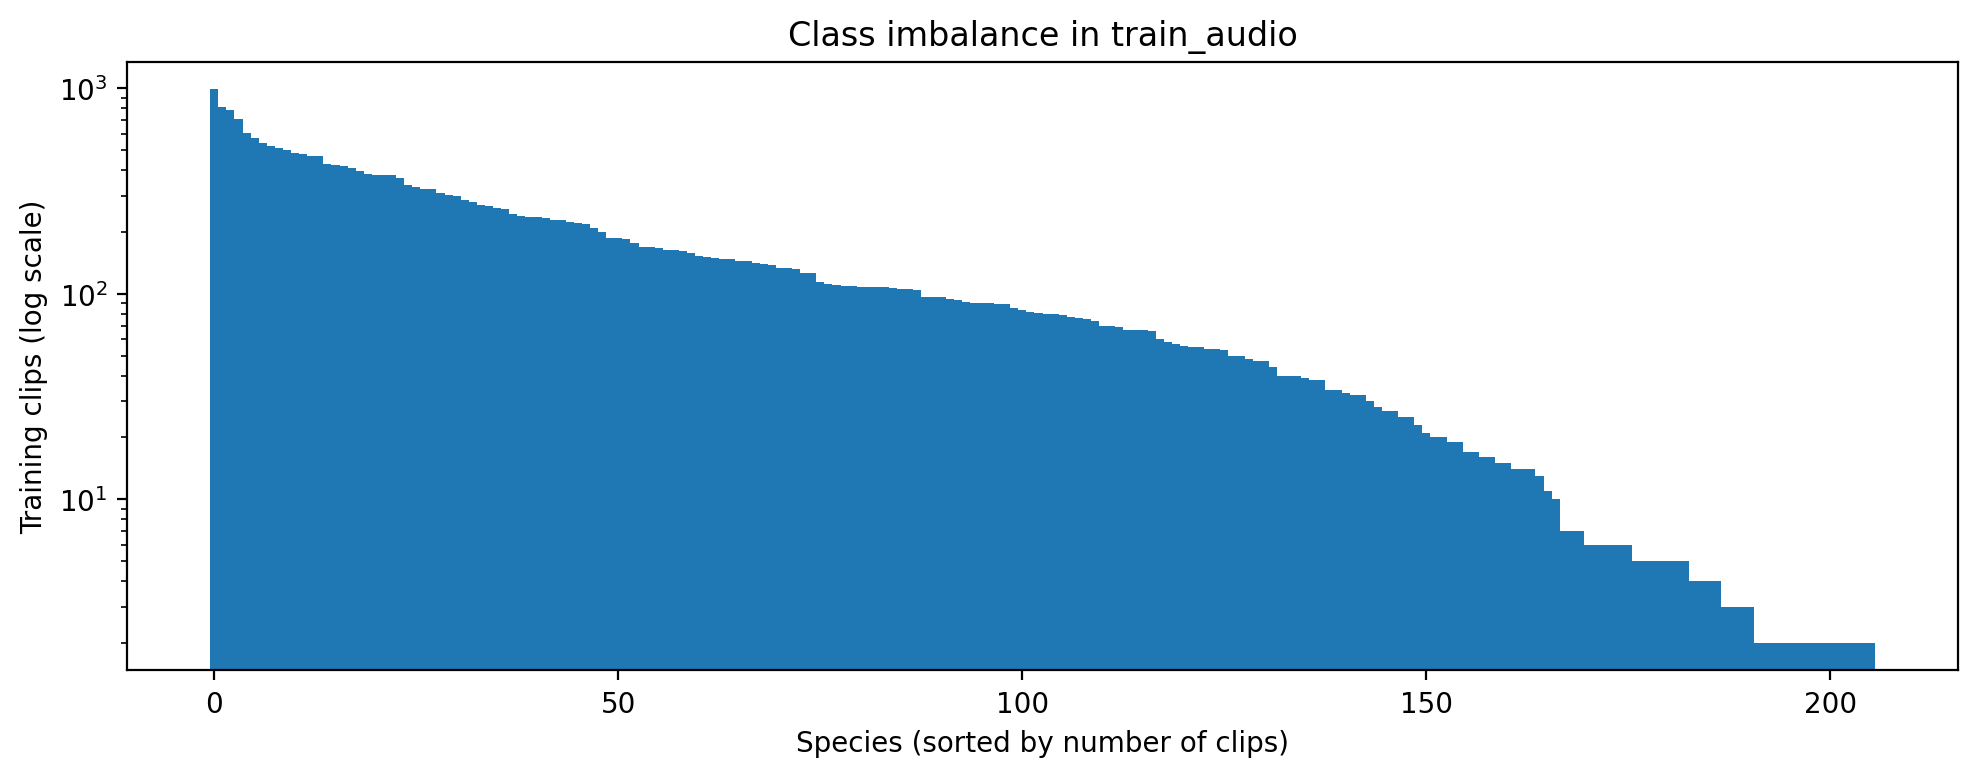
\includegraphics[width=\columnwidth]{figures/class_imbalance.png}
\caption{Training clips per species, sorted. The long tail of rare species matters because every species counts equally in macro ROC-AUC.}
\label{fig:imbalance}
\end{figure}

\begin{figure*}[t]
\centering
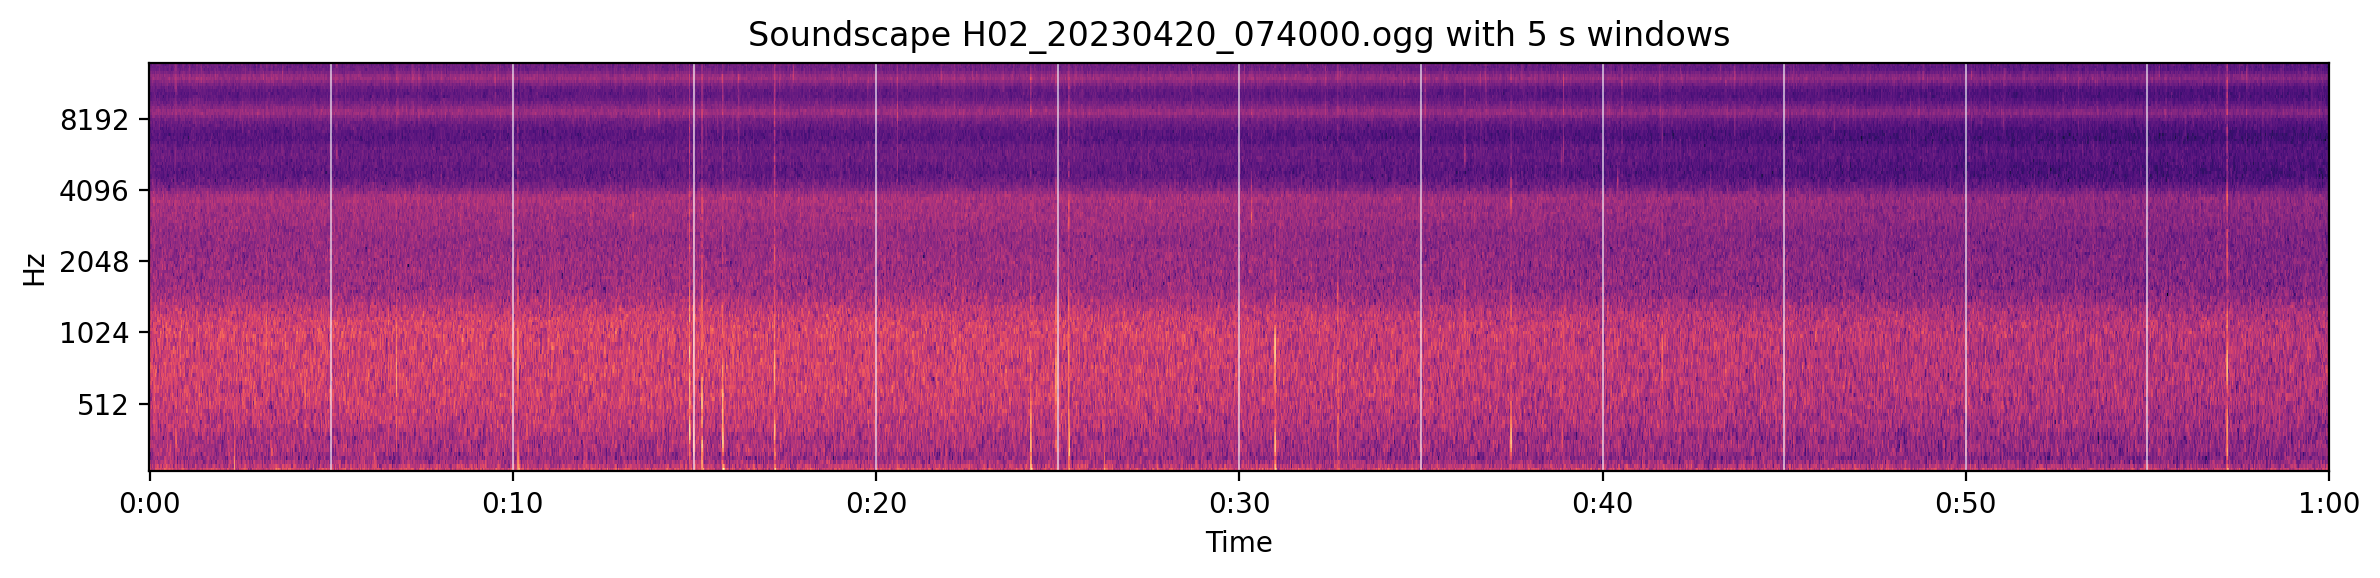
\includegraphics[width=0.9\textwidth]{figures/soundscape_windows.png}
\caption{An unlabelled 60\,s training soundscape from a field recorder, split into the twelve 5\,s windows that must each be scored. Unlike the close-up focal training clips, calls are faint and short against continuous background noise.}
\label{fig:soundscape}
\end{figure*}

\section{Methodology}
\label{sec:method}
Every model outputs 206 sigmoid probabilities per 5\,s window. Figure~\ref{fig:arch} shows the final system; the components are introduced in the order we built them.

\begin{figure*}[t]
\centering
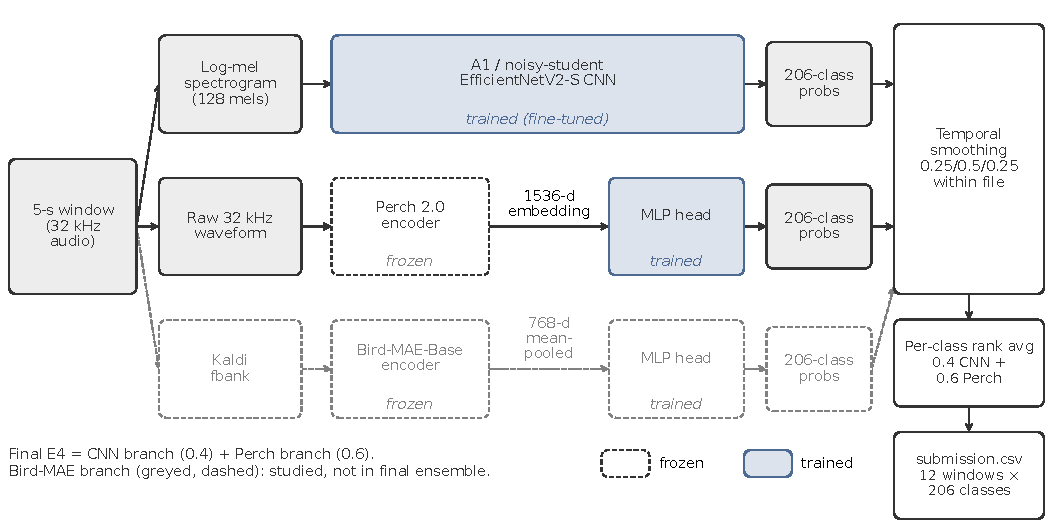
\includegraphics[width=0.92\textwidth]{figures/fig_f1_architecture.pdf}
\caption{Final system. A 5\,s window is scored by a log-mel CNN (bird-pretrained EfficientNetV2-S, trained as a noisy student) and by frozen Perch 2.0 followed by a trained MLP head (distilled from the CNN, ``A2d''). Window probabilities are smoothed over neighbouring windows and combined by a per-class rank average with weights 0.4/0.6. The greyed Bird-MAE branch was studied but is not in the final ensemble.}
\label{fig:arch}
\end{figure*}

\subsection{Input features and baseline}
Audio is converted to 128-band log-mel spectrograms (FFT 2048, hop 512, i.e.\ 16\,ms per frame, 50--14,000\,Hz) with librosa \citep{mcfee2015librosa}. We use spectrograms because they turn audio into an image, which lets us reuse ImageNet-pretrained CNNs \citep{deng2009imagenet}, an important help when some species have two clips. The lower limit removes wind and handling rumble; the upper limit keeps high-pitched insects below the Nyquist frequency. Each window is converted to decibels relative to its own maximum, clipped to an 80\,dB range and scaled to $[0,1]$, so quiet, distant calls in the soundscapes and loud focal calls share one scale.

The \textbf{baseline} classifies the first 5\,s of each clip with EfficientNet-B0 \citep{tan2019efficientnet} (ImageNet weights, one input channel, 4.3\,M parameters with 206 outputs) using binary cross-entropy (BCE), because several species can call at once and the metric scores each separately. We chose the smallest EfficientNet so that several models could later fit into the CPU budget. Training uses AdamW \citep{loshchilov2019decoupled} (learning rate $10^{-3}$, weight decay $10^{-2}$) with a one-cycle schedule \citep{smith2019super}, batch 64, 15 epochs, on a stratified 80/20 split (seed 42; 22,851/5,713 clips). Validation AUC is computed on the first 5\,s of each hold-out clip against its primary label. At test time each soundscape is cut into twelve windows and scored on CPU.

\subsection{Baseline improvements (baseline v2)}
To sample any part of a recording, we cache whole-clip spectrograms (up to 30\,s) once as 8-bit integers over a 120\,dB range (35.6\,M frames, 4.6\,GB) and normalise each cut window exactly as at test time (99th-percentile error 0.005 against spectrograms computed from audio). This pipeline alone reproduces the baseline (validation 0.971 vs.\ 0.973) and halves training time. We then test one change per difficulty:
\begin{itemize}
\item \textbf{Random crop} (weak labels): a random 5\,s window of the whole clip instead of the first 5\,s.
\item \textbf{Soundscape noise + mixup} (domain shift): with probability 0.5 a random window of an unlabelled soundscape is added at $-20$ to $-3$\,dB; with probability 0.5 two samples are mixed with Beta(0.4,\,0.4) weights and the target is the element-wise maximum \citep{zhang2018mixup}.
\item \textbf{Secondary labels} (label noise): secondary species get a soft target of 0.5 instead of 0.
\item \textbf{Focal loss} (imbalance): BCE is replaced by focal loss with $\gamma=2$ \citep{lin2017focal}.
\end{itemize}
Baseline \textbf{v2} combines the changes that raised the public score (crop, noise/mixup, secondary labels) and is the starting point of every later model.

\subsection{Sound event detection model}
The baseline scores each window as a whole and cannot tell \emph{when} in a weakly labelled clip a species calls. An SED model predicts a score for every short time step and pools them into one clip score for training, so it learns call timing from clip labels alone \citep{mesaros2021sound,kong2020panns}. We re-implemented the SED approach described in the first-place write-up \citep{babych2025first}, whose head goes back to a 2021 solution \citep{tattaka2021fourth}, from the written descriptions only.

The input is a 20\,s chunk ($128\times1251$). We keep the v2 EfficientNet-B0 but remove its pooling and classifier, so the time axis survives ($1280\times4\times40$; 0.5\,s per step), which means any change in score comes from the head and chunk length, not a larger backbone. Generalised-mean pooling \citep{radenovic2019finetuning} with $p=3$ collapses frequency: a call fills few bands, so average pooling would dilute it and max pooling would follow noisy peaks. A shared $1\times1$ convolution (512 channels, ReLU, dropout 0.25) feeds two $1\times1$ heads, giving a score and an attention weight (softmax over time) for each species and step (Figure~\ref{fig:sed}). The score bias starts at $-4$ because nearly every species is absent at nearly every step. The loss is $0.5\,\mathrm{BCE}(\text{attention-pooled}) + 0.5\,\mathrm{BCE}(\text{max over time})$; the max term trains the step scores directly, which are what we use at test time. Training applies the full v2 recipe to random 20\,s chunks. At inference, 20\,s chunks start every 5\,s; each window takes its highest step score and averages over the up to four chunks covering it. A second model is trained identically on 5\,s chunks to measure what the long context is worth.

\begin{figure}[t]
\centering
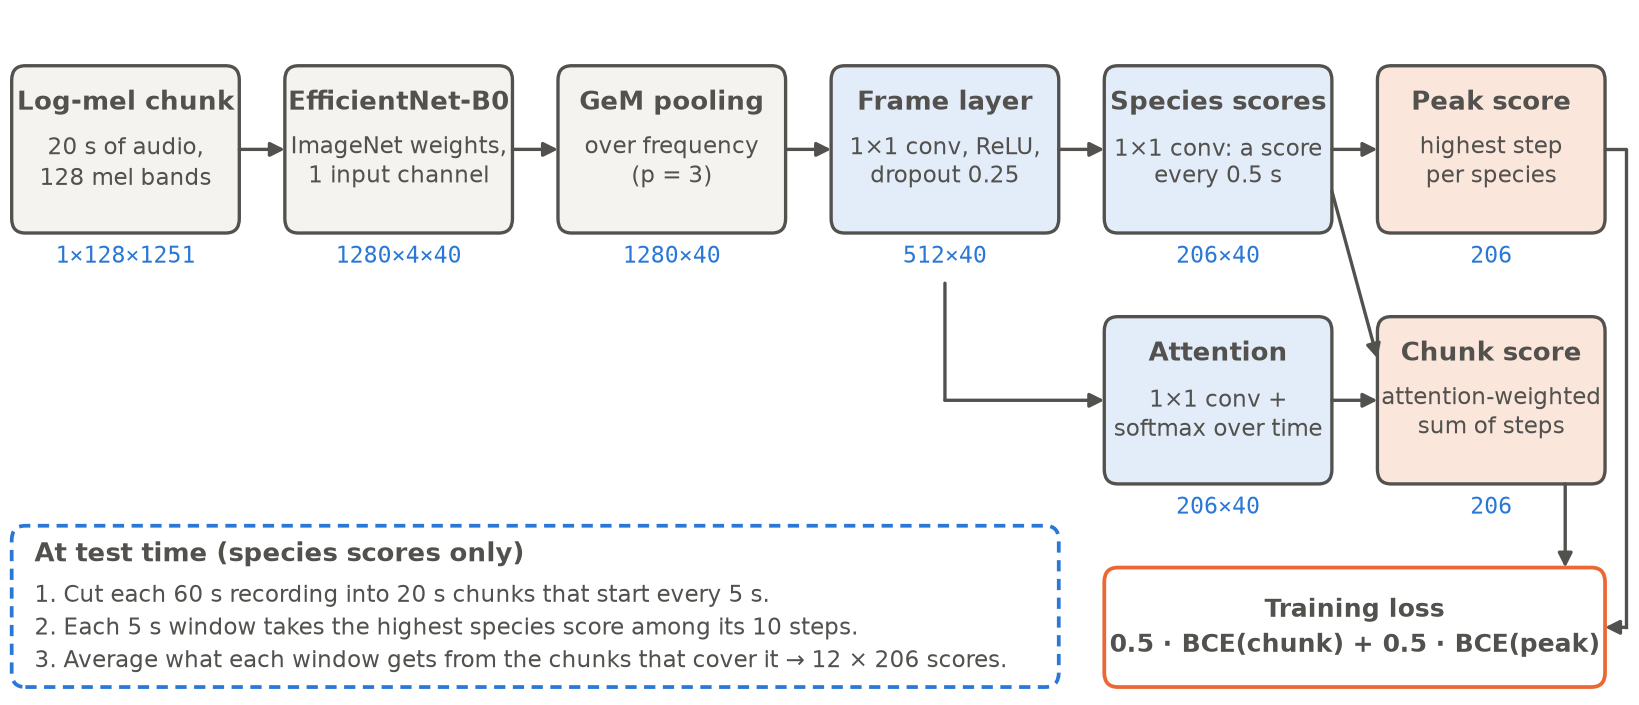
\includegraphics[width=\columnwidth]{figures/sudhishna_sed_architecture.png}
\caption{SED model. Tensor shapes are for one 20\,s chunk (channels $\times$ frequency $\times$ time). The head turns EfficientNet-B0 features into per-step species scores and attention weights; attention- and max-pooled scores form the training loss.}
\label{fig:sed}
\end{figure}

\subsection{Pretrained models}
Keeping v2's recipe, split and inference fixed, we change only the pretrained model.
\textbf{A1 (supervised bird CNN)} fine-tunes the bird-pretrained \texttt{tf\_efficientnetv2\_s\_in21k} backbone released by the second-place team \citep{sydorskyi2025tackling} end to end with v2's recipe (774 of 780 weight tensors loaded; the last convolution and batch-norm start random).
\textbf{A2 (frozen multi-taxa)} freezes Perch 2.0 \citep{vanmerrienboer2025perch}, run on CPU through a community ONNX conversion \citep{calotriton2025perchonnx}, embeds up to 30\,s of each clip (106,157 windows) and trains an MLP head (512 hidden units, dropout 0.3) with targets 1.0 (primary) and 0.5 (secondary), each window weighted by one over its clip's window count.
\textbf{A3 (frozen self-supervised)} does the same with Bird-MAE-Base \citep{rauch2025can} (ViT-B/16, 768-d mean-pooled tokens) and its own filterbank front end.

\subsection{Label-free adaptation}
No soundscape labels exist, so all adaptation uses unlabelled \texttt{train\_soundscapes} audio. We compare two families.
\emph{Statistics-level} methods change how features are scaled. AdaBN resets and re-estimates all batch-norm statistics on 12,000 soundscape windows from 1,000 files \citep{li2018adaptive}. For frozen embeddings, mean/std matching maps focal embeddings to the soundscape mean and standard deviation per dimension, and standardised CORAL \citep{sun2016return} additionally whitens with the focal and re-colours with the soundscape correlation matrix (ridge 1.0); the head is then trained on the mapped focal embeddings.
\emph{Content-level} methods change what the model is trained on. In \textbf{head distillation}, a teacher labels the 12,000 soundscape windows; probabilities $p$ are sharpened to $p^{1.3}$ and values below 0.01 set to 0, and the student head trains on the real labels plus these windows at loss weight 0.5. We ran two pairs, Perch head $\rightarrow$ Bird-MAE head (A3d) and, across model families, A1 CNN $\rightarrow$ Perch head (\textbf{A2d}). In the \textbf{noisy student} round (Figure~\ref{fig:ns}), a teacher labels all 116,712 windows of the 9,726 soundscapes and a fresh bird-pretrained V2-S student is trained on the focal clips plus 30,000 pseudo-labelled windows per epoch (loss weight 0.5), with mixup and stochastic depth 0.15 \citep{huang2016deep} as noise. The MAIN teacher is the mean of A1 and A2; the ABLATION teacher is A2d alone.

\begin{figure*}[t]
\centering
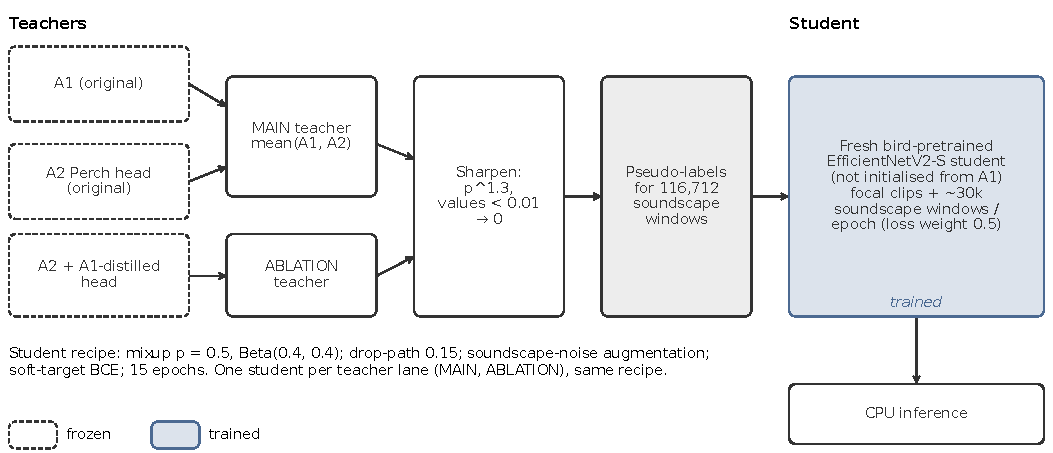
\includegraphics[width=0.86\textwidth]{figures/fig_f4_noisy_student.pdf}
\caption{Noisy student, round 1. Teachers (MAIN: mean of A1 and A2; ABLATION: A2d) label all 116,712 soundscape windows; labels are sharpened and a freshly initialised bird-pretrained EfficientNetV2-S student is trained on focal clips plus pseudo-labelled windows. No soundscape label is used anywhere.}
\label{fig:ns}
\end{figure*}

\subsection{Ensemble and CPU inference}
Each model's probabilities are smoothed within a file, $p'_t = 0.25\,p_{t-1} + 0.5\,p_t + 0.25\,p_{t+1}$ (renormalised at the ends), because calls often span window borders. Models are then combined by a per-class weighted rank average, $s_{r,c}=\sum_m w_m\,\mathrm{rank}_c(p^{(m)}_{r,c})/\sum_m w_m$, with ranks scaled to $[0,1]$. ROC-AUC depends only on the order within a class, so averaging ranks removes the different probability scales of a CNN and an MLP head. To fit two models into 90 CPU minutes we profiled v2's inference and found mel computation to be the largest cost; the fast pipeline uses four file-level workers, one mel call per file and one batch per file, which cut v2 from 11.1 to 5.5 minutes for 700 files.

\section{Experiments}
\begin{table}[t]
\centering
\small
\begin{tabular}{lc}
\toprule
Head (frozen encoder) & Val AUC, mean $\pm$ std \\
\midrule
A2 Perch head & 0.99163 $\pm$ 0.00029 \\
A3 Bird-MAE head & 0.97451 $\pm$ 0.00076 \\
A2d (A1-distilled) & 0.99133 $\pm$ 0.00047 \\
A3d (A2-distilled) & 0.97506 $\pm$ 0.00012 \\
\bottomrule
\end{tabular}
\caption{Seed repeats of the MLP heads (seeds 42--44, split fixed). Seed noise in validation is at most 0.0008, far smaller than the leaderboard effects we report.}
\label{tab:seed}
\end{table}

\paragraph{Protocol.} All runs use v2's split, seed and recipe; training ran on Kaggle T4 GPUs and inference on Kaggle CPU with internet off. Every variant was submitted once. We quote public-leaderboard scores in the text, as the public leaderboard is used for comparison and grading; the tables also list private scores for completeness. Repeating the small heads over three seeds changed validation AUC by at most 0.0008 (Table~\ref{tab:seed}), so the effects below are not seed noise on the validation side; leaderboard noise could not be measured without repeated submissions. Following our ablations, we treat public differences below 0.01 as noise and select by the public score, because clean focal validation did not predict the leaderboard (Section~\ref{sec:disc}). Variants and selection rules for the adaptation, distillation and ensemble phases were written down before their scores; the exceptions are stated in the Limitations.

\subsection{Baseline and ablations}
The baseline reaches a validation AUC of 0.973 at epoch 7 and then overfits (0.960 at epoch 15) while training loss falls towards zero. On the leaderboard it scores only 0.71681 public, the first sign of the domain shift. Table~\ref{tab:ablation} and Figure~\ref{fig:ablation} add one change at a time and then remove one from v2.

\begin{table}[t]
\centering
\small
\begin{tabular}{lcccc}
\toprule
Run & Val & Public & Private & $\Delta$ pub. \\
\midrule
Baseline & 0.973 & 0.717 & 0.699 & -- \\
+ random crop & 0.982 & 0.752 & 0.754 & $+0.035$ \\
+ noise / mixup & 0.975 & 0.732 & 0.733 & $+0.016$ \\
+ secondary labels & 0.969 & 0.729 & 0.733 & $+0.012$ \\
+ focal loss & 0.973 & 0.705 & 0.710 & $-0.012$ \\
\midrule
\textbf{v2} (crop+noise+sec.) & 0.977 & \textbf{0.763} & \textbf{0.789} & $+0.046$ \\
v2 $-$ random crop & 0.974 & 0.753 & 0.772 & $-0.010$ \\
v2 $-$ noise / mixup & 0.981 & 0.767 & 0.760 & $+0.004$ \\
v2 $-$ secondary labels & 0.979 & 0.737 & 0.772 & $-0.026$ \\
v2 + focal loss & 0.978 & 0.743 & 0.782 & $-0.020$ \\
\bottomrule
\end{tabular}
\caption{Ablations of the baseline (top, $\Delta$ vs.\ baseline) and of v2 (bottom, $\Delta$ vs.\ v2). Val is best-epoch validation AUC on hold-out focal clips; public/private are leaderboard AUC.}
\label{tab:ablation}
\end{table}

\begin{figure}[t]
\centering
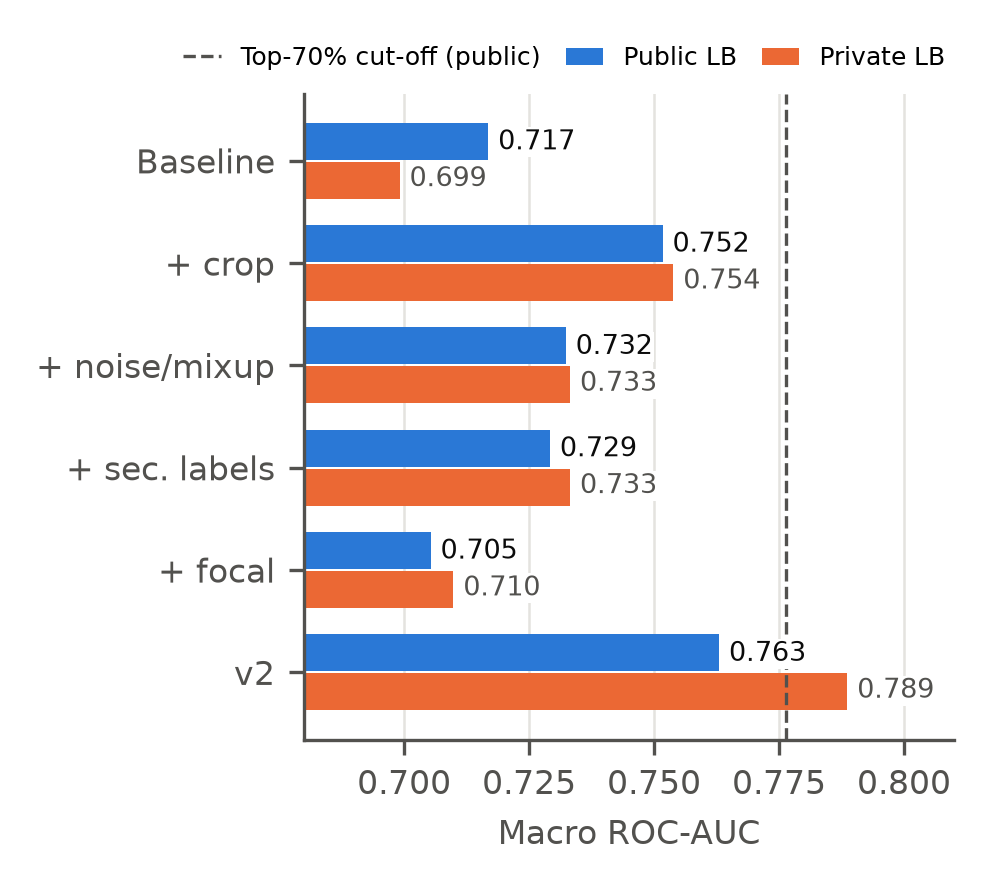
\includegraphics[width=0.82\columnwidth]{figures/jamie_ablation_single.png}
\caption{Leaderboard AUC when one change is added to the baseline, and the combined v2. The dashed line is the public top-70\% cut-off.}
\label{fig:ablation}
\end{figure}

Random crops give the largest single gain ($+0.035$ public): many first-5\,s windows hold no call, and sampling the whole clip fixes this. They also act as augmentation; the crop and noise runs are still at or near their best at epoch 15 instead of overfitting at epoch 5 to 7. Noise/mixup and secondary labels help less on the hold-out clips than on the leaderboard, as expected for changes that target soundscapes. Focal loss does not help ($-0.012$ public). In the remove-one study, secondary labels matter most once combined ($-0.026$ when removed, against $+0.012$ alone); a likely reason is that random crops often contain background species, and secondary labels give those windows correct targets. Removing noise/mixup raises the public score slightly ($+0.004$, within noise) but costs 0.028 private, so we keep it. v2 reaches 0.763 public, $+0.046$ over the baseline.

\subsection{SED model}
Table~\ref{tab:sed} lists the SED runs. On 20\,s chunks SED stays below v2; the best 20\,s run is 0.015 public below v2. Keeping the final instead of the best-validation epoch raised the score by 0.013 to 0.016 public: at the validation peak (epoch 7) the one-cycle learning rate was still 64\% of its maximum, so the clean hold-out was again a poor guide. Overlapping chunks helped every time (public $+0.006$ to $+0.012$, all six differences with the same sign) for about 7 extra CPU minutes. The first-place spectrogram settings (224 bands, 1.25\,s steps) did not help. The largest effect was the \textbf{chunk length}: the same model on 5\,s chunks scored $+0.033$ public over 20\,s chunks, drawing level with v2 (0.773 vs.\ 0.763) at an estimated 16 CPU minutes. So the SED head works and the 20\,s chunk held it back, the opposite of the first-place finding. Our likely explanation, untested, is padding: 47.9\% of our clips are shorter than 20\,s, so many 20\,s training chunks are mostly silence, unlike the test soundscapes. Trained only with clip labels, the model's step scores still rise exactly when the species calls on hold-out clips (Figure~\ref{fig:frames}).

\begin{table}[t]
\centering
\small
\begin{tabular}{lccc}
\toprule
Run (weights; chunk start) & Val & Public & Private \\
\midrule
v2 (CNN, 5\,s windows) & 0.977 & 0.763 & 0.789 \\
SED 20\,s (best ep.; every 20\,s) & 0.970 & 0.726 & 0.744 \\
\quad + overlap (every 5\,s) & 0.970 & 0.732 & 0.752 \\
\quad + final epoch & 0.974 & 0.740 & 0.749 \\
\quad + final epoch + overlap & 0.974 & 0.748 & 0.763 \\
\quad + 224-band mels & 0.972 & 0.728 & 0.755 \\
\quad + 224-band + overlap & 0.972 & 0.740 & 0.761 \\
\textbf{SED 5\,s} (final epoch) & 0.980 & \textbf{0.773} & 0.787 \\
\bottomrule
\end{tabular}
\caption{SED runs; all use the v2 recipe. Val is first-5\,s hold-out AUC. ``Overlap'' starts a 20\,s chunk every 5\,s and averages the windows' scores.}
\label{tab:sed}
\end{table}

\begin{figure}[t]
\centering
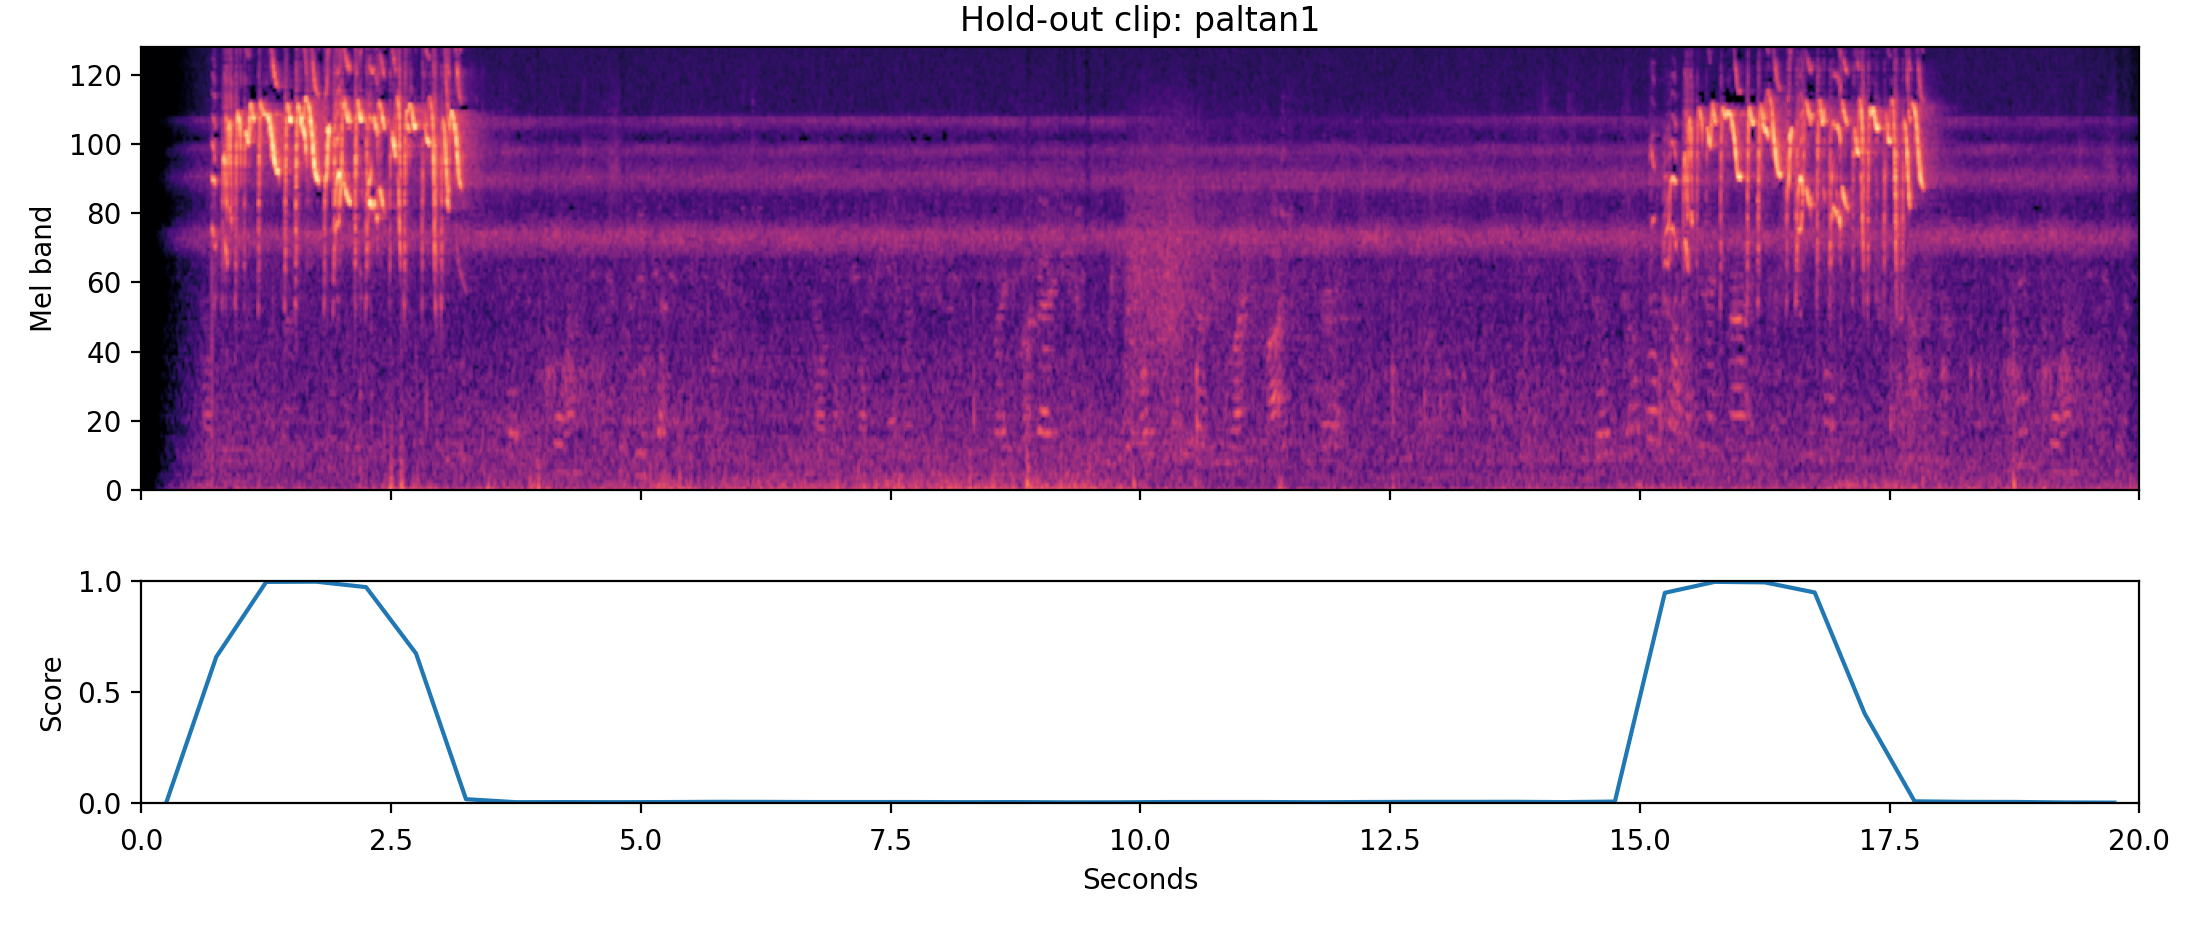
\includegraphics[width=\columnwidth]{figures/sudhishna_frame_scores.png}
\caption{A hold-out clip of one species (top) and the SED model's score for it every 0.5\,s (bottom). Although trained only with clip-level labels, the score rises when the species calls.}
\label{fig:frames}
\end{figure}

\subsection{Pretrained models}
Table~\ref{tab:base} compares the three paradigms with v2. Perch 2.0 is best ($+0.085$ public over v2) and the bird CNN second ($+0.065$). Bird-MAE gains only $+0.013$ public, close to our noise threshold and not confirmed on the private part, so we do not read it as an improvement. All models have a \emph{transfer gap} (validation minus public AUC) of 0.14 to 0.21: clean validation ranks them in the leaderboard order but compresses the spread (0.017 against 0.071).

\begin{table}[t]
\centering
\small
\begin{tabular}{lccccc}
\toprule
Model & Val & Public & Private & Gap & CPU \\
\midrule
v2 (B0, ImageNet) & 0.977 & 0.763 & 0.789 & .214 & 11.1 \\
A1 V2-S, bird & 0.983 & 0.828 & 0.816 & .155 & 8.0 \\
A2 Perch 2.0 & 0.992 & \textbf{0.848} & \textbf{0.852} & .144 & 25.0* \\
A3 Bird-MAE & 0.975 & 0.776 & 0.780 & .199 & 61.6* \\
\bottomrule
\end{tabular}
\caption{Pretraining paradigms, one submission each. Gap = Val $-$ public. CPU = minutes for 700 files, measured (v2: original pipeline; A1: fast pipeline) or *projected from a 20-file dry run.}
\label{tab:base}
\end{table}

\subsection{Label-free adaptation}
Table~\ref{tab:adapt} lists every adaptation submission against its unadapted parent. \textbf{Statistics-level alignment lowered the public score in all seven cases}, by 0.024 to 0.161, although focal validation AUC barely moved (Perch 0.9916 to 0.9901). The loss was largest for frozen embeddings. A control run of the unadapted A1 through the same fast notebook reproduced its original score exactly, so the AdaBN drop is not a pipeline error. \textbf{Content-level adaptation raised the public score in all four cases}, by 0.012 to 0.036, and narrowed the transfer gap each time (Figure~\ref{fig:gap}). A2d learned from the \emph{weaker} A1 teacher (0.828 vs.\ A2's 0.848) and still improved, becoming our best single model (0.86651 public). Distillation combined with CORAL recovered only part of the CORAL loss, so the damage from the mapping survives pseudo-labels.

\begin{table}[t]
\centering
\footnotesize
\setlength{\tabcolsep}{4pt}
\begin{tabular}{llcccc}
\toprule
Parent & Method & Public & $\Delta$pub. & Private & $\Delta$priv. \\
\midrule
v2 & AdaBN & 0.739 & $-0.024$ & 0.764 & $-0.025$ \\
A1 & AdaBN & 0.772 & $-0.056$ & 0.766 & $-0.051$ \\
A2 & CORAL & 0.688 & $-0.160$ & 0.709 & $-0.144$ \\
A2 & mean/std & 0.687 & $-0.161$ & 0.706 & $-0.146$ \\
A3 & CORAL & 0.643 & $-0.134$ & 0.647 & $-0.133$ \\
A3 & mean/std & 0.670 & $-0.107$ & 0.680 & $-0.100$ \\
A3 & distil.+CORAL & 0.693 & $-0.083$ & 0.689 & $-0.092$ \\
\midrule
A3 & A2-distil.\ (A3d) & 0.812 & $+0.036$ & 0.802 & $+0.022$ \\
A2 & A1-distil.\ (A2d) & \textbf{0.867} & $+0.019$ & \textbf{0.857} & $+0.005$ \\
A1 & NS MAIN & 0.860 & $+0.032$ & 0.852 & $+0.035$ \\
A1 & NS ABLATION & 0.840 & $+0.012$ & 0.838 & $+0.022$ \\
\bottomrule
\end{tabular}
\caption{Adaptation with unlabelled soundscapes against the unadapted parent. Top: statistics-level; bottom: content-level (NS = noisy student). The A2d private change is within noise.}
\label{tab:adapt}
\end{table}

\begin{figure}[t]
\centering
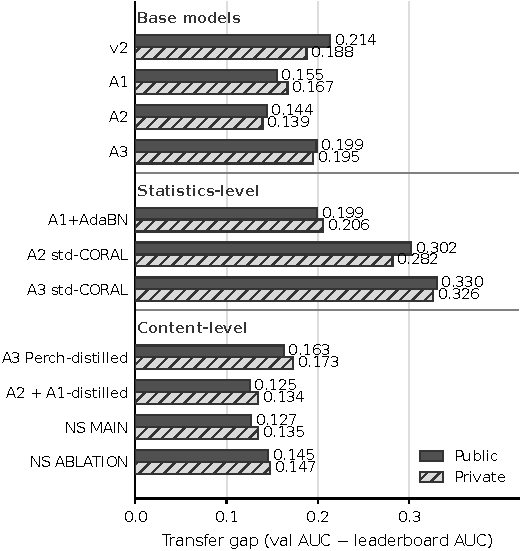
\includegraphics[width=0.82\columnwidth]{figures/fig_transfer_gap.pdf}
\caption{Transfer gap (validation AUC minus leaderboard AUC; dark public, hatched private) of the base models, three statistics-level variants and the four content-level models. Statistics alignment widened the gap; pseudo-labels narrowed it.}
\label{fig:gap}
\end{figure}

\paragraph{Noisy student.} MAIN beats ABLATION by $+0.020$ public and gains $+0.032$ public over its initialisation A1 at almost the same CPU cost (9.9 vs.\ 8.0 minutes). The two arms differ in teacher \emph{and} label density (2.50\% vs.\ 0.74\% non-zero labels), so the difference cannot be assigned to the teacher alone. Their validation curves end within 0.002 of each other, so validation could not have chosen between them.

\subsection{Ensemble and final submission}
Table~\ref{tab:ens} shows the ensembles of the MAIN student and A2d. E1 beats the best single model by $+0.017$ public, so the CNN and the Perch head are complementary: the per-class Spearman correlation of A1 and A2 probabilities on soundscape windows is only 0.31. Smoothing adds a further $+0.003$ public. Adding the ABLATION student (E3) moved weight away from Perch and lowered the public score. E4 (0.4 CNN / 0.6 Perch) was the pre-registered pick by public score; it and E2 are within noise. Figure~\ref{fig:lb} summarises the progression.

\begin{table}[t]
\centering
\small
\begin{tabular}{llccc}
\toprule
 & Weights; smoothing & Public & Private & CPU \\
\midrule
E1 & .5/.5; no & 0.88352 & 0.87203 & 28.3 \\
E2 & .5/.5; yes & 0.88662 & 0.88008 & 30.4 \\
E3 & 1/3 each (+ABL.); yes & 0.88058 & 0.87522 & 39.9 \\
\textbf{E4} & .4/.6; yes & \textbf{0.88749} & \textbf{0.88029} & 32.3 \\
\bottomrule
\end{tabular}
\caption{Rank-average ensembles of the noisy-student MAIN CNN and A2d (weights in that order). CPU minutes measured on 700 files (limit 90).}
\label{tab:ens}
\end{table}

\begin{figure*}[t]
\centering
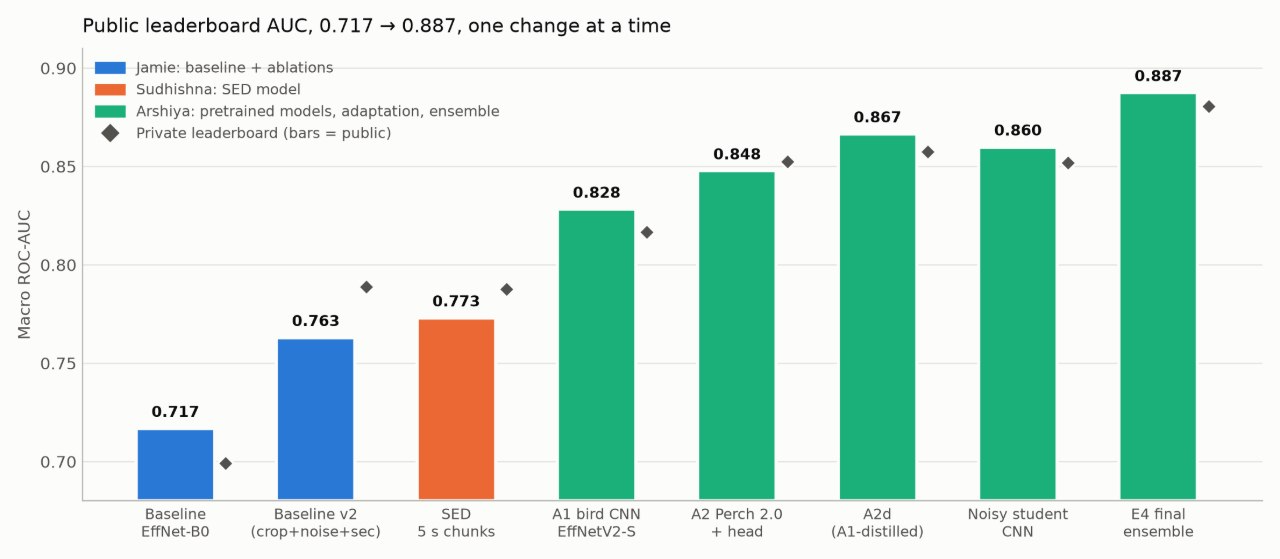
\includegraphics[width=0.9\textwidth]{figures/progression_by_member.png}
\caption{Public leaderboard AUC (bars) and private AUC (diamonds) of the main systems in the order they were built, coloured by the member who built them: from the baseline (0.717) to the final ensemble E4 (0.887), one change at a time. Each value is one late submission.}
\label{fig:lb}
\end{figure*}

\paragraph{Leaderboard position.} Table~\ref{tab:rank} places our main milestones in the public leaderboard of 2,032 teams. Because late submissions are unranked, the position is the rank our score would take; Figures~\ref{fig:score} and~\ref{fig:position} show the score and the corresponding place in the leaderboard. E4 (0.88749) falls between rank 72 (0.88753) and rank 73 (0.88745), a relative ranking of $73/2032 = 3.6\%$, inside the top-10\% band (cut-off 0.8808). For reference, the best public score is 0.93376, so E4 is 0.046 below the top of the public leaderboard.

\begin{table}[t]
\centering
\small
\begin{tabular}{lccc}
\toprule
System & Public & Position & Relative \\
\midrule
Baseline & 0.71681 & 1600 & 78.7\% \\
Baseline v2 & 0.76299 & 1481 & 72.9\% \\
SED 5\,s & 0.77298 & 1427 & 70.2\% \\
A2d (best single) & 0.86651 & 647 & 31.8\% \\
\textbf{E4 (final)} & \textbf{0.88749} & \textbf{73} & \textbf{3.6\%} \\
\bottomrule
\end{tabular}
\caption{Position each score would take in the BirdCLEF+ 2025 public leaderboard (2,032 teams) and relative ranking (position / 2,032).}
\label{tab:rank}
\end{table}

\begin{figure}[t]
\centering
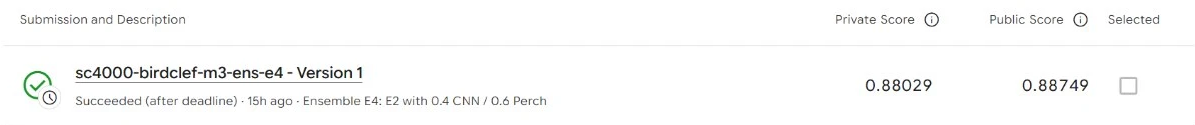
\includegraphics[width=\columnwidth]{figures/kaggle_e4_score.png}
\caption{Kaggle submission page for the final ensemble E4: 0.88749 public, 0.88029 private (late submission).}
\label{fig:score}
\end{figure}

\begin{figure}[t]
\centering
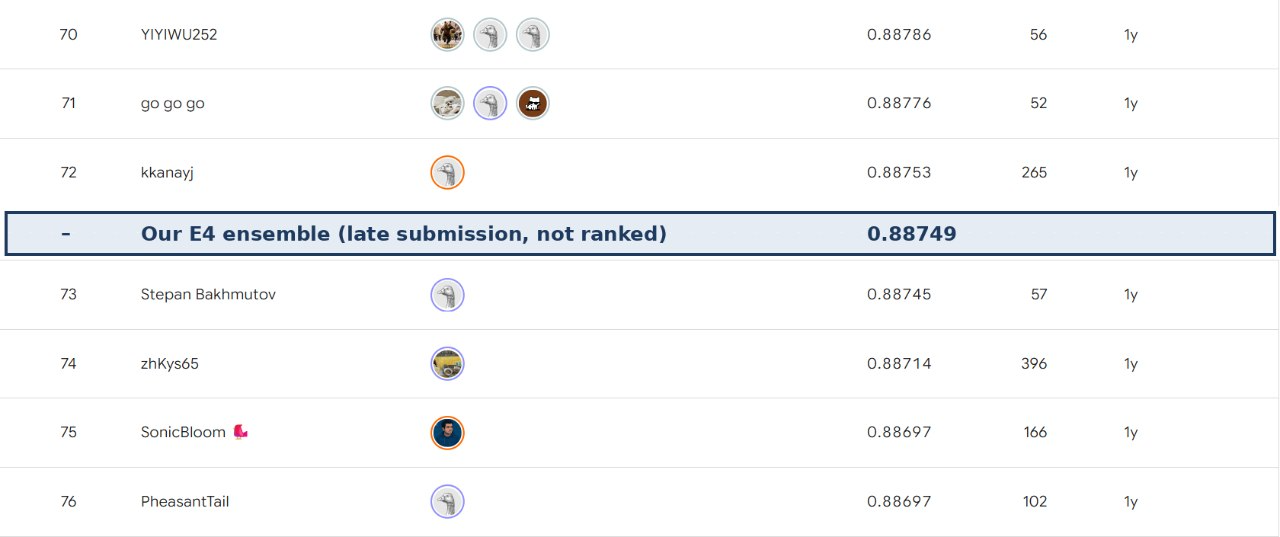
\includegraphics[width=\columnwidth]{figures/kaggle_e4_leaderboard_position.png}
\caption{BirdCLEF+ 2025 public leaderboard, ranks 70--76. The highlighted row, added by us, marks where our late E4 score (0.88749) falls: between rank 72 (0.88753) and rank 73 (0.88745) of 2,032.}
\label{fig:position}
\end{figure}

\section{Discussion}
\label{sec:disc}
\paragraph{Clean validation does not predict the leaderboard.} This is the common thread of all three parts of the project. In the ablations, v2 without noise has the highest validation AUC of the v2 runs but the lowest private score, and secondary labels lower validation AUC while raising the leaderboard score. In the SED runs, keeping the best-validation epoch cost up to 0.016 public. Among pretrained models, validation spans 0.017 while public scores span 0.071, and AdaBN/CORAL hardly changed validation while losing up to 0.16 on the leaderboard. Figure~\ref{fig:cvlb} shows the ablation runs. Hold-out focal clips come from the training distribution and cannot measure robustness to soundscapes, which is why we selected by public score and treated differences below 0.01 as noise.

\begin{figure}[t]
\centering
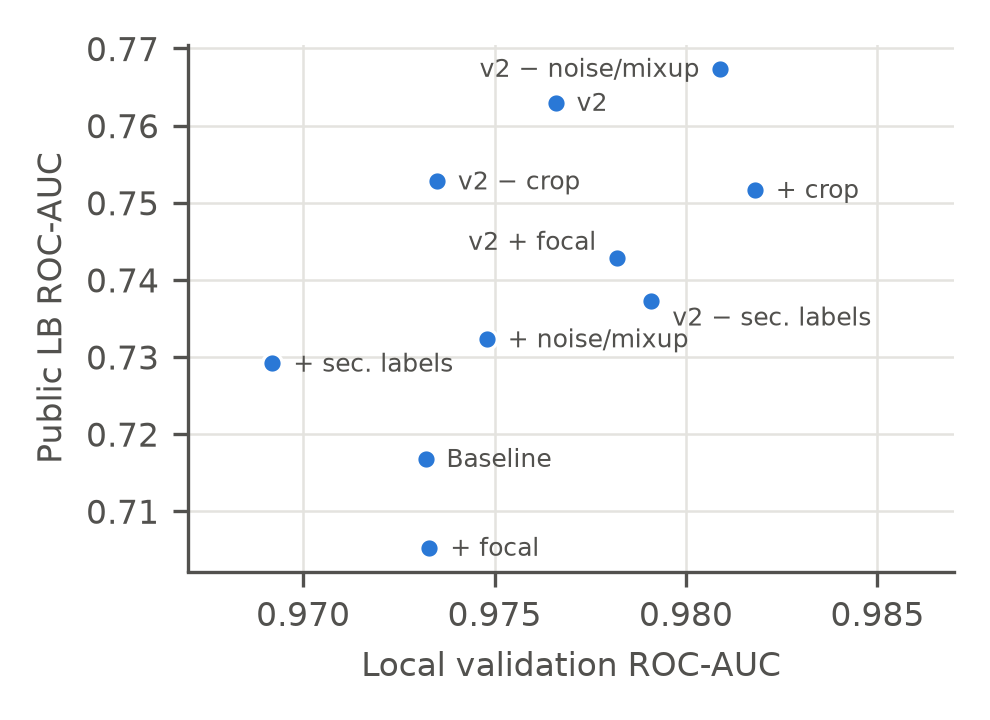
\includegraphics[width=0.85\columnwidth]{figures/jamie_cv_vs_lb.png}
\caption{Validation AUC on clean hold-out clips against public leaderboard AUC for the ten baseline-ablation runs. The two are only weakly related.}
\label{fig:cvlb}
\end{figure}

\paragraph{Why statistics alignment failed.} A diagnostic notebook found no pipeline bug (CORAL and original inference paths differ by at most $3\times10^{-8}$ with the original head). Our pre-registered explanation, that adapted heads assign much higher probabilities to background windows, is not supported: the mean probability on 12,000 soundscape windows rose for only one variant. What changed instead was the \emph{ranking} within each class (per-class Spearman correlation with the original head 0.29 to 0.37 for Perch), and ROC-AUC is sensitive to exactly this. A plausible but untested cause is that soundscape statistics are dominated by windows with no target species, so aligning to them moves call-bearing clips toward background.

\paragraph{Why pseudo-labels helped.} Content-level adaptation changes what the model sees rather than how its features are scaled: pseudo-labelled soundscape windows show the student real background, including that most windows hold no target species, while soft labels carry the teacher's knowledge. A2d improving from a weaker teacher of another family suggests the gain comes from complementary errors rather than teacher strength, in line with the motivation for cross-lineage teachers \citep{farazi2026crossmutated}; two runs are too few to prove it.

\paragraph{Bird-MAE and a misleading probe.} A linear probe on Bird-MAE features first reached only 0.750 validation AUC, with a first-epoch loss near $\ln 2$. Initialising the output bias to the class log-prior \citep{lin2017focal}, with nothing else changed, gave 0.963, so the default probe measured its initialisation rather than the features. Even after this fix, Bird-MAE transferred worst; mean-pooling 256 patch tokens may dilute short calls, and a self-supervised, bird-only objective may separate 60 non-bird classes less well. We did not test these hypotheses.

\paragraph{Speed.} In E4 the Perch encoder is about 73\% of the summed CPU time; the whole notebook ran in 32.3 minutes, well under the 90-minute limit, whereas Bird-MAE (61.6 projected minutes) would have left little room for a second model.

\paragraph{Limitations.} We used one split; CNNs were trained once and only the small heads were repeated over seeds (validation standard deviation at most 0.0008). The 0.01 noise threshold was not measured by repeated submissions, and public and private parts disagree on some close calls. The noisy-student MAIN teacher was chosen after the A2d score was known, and the A1 control was requested after the AdaBN score. Perch 2.0 was released in August 2025, after the competition closed, so A2, A2d and the ensemble are not comparable to official entries, and Perch's training data may overlap with \texttt{train\_audio}. Without labelled soundscapes we could not test the domain-shift explanations directly.

\section{Future Work}
Four directions follow from our results. First, a small labelled soundscape set would give a validation signal that matches the test data, which every part of this project lacked, and would allow per-taxon evaluation of our hypotheses. Second, the first-place solution ran several noisy-student rounds; we ran one, so more rounds, with pseudo-label filtering by confidence or teacher agreement and a density-matched control, would show whether the gain compounds and separate teacher quality from label density. Third, the 5\,s SED model scores level with v2 but is a different kind of model, so adding it, or an SED head on the bird-pretrained backbone, to the ensemble is a cheap next step (16 CPU minutes). Fourth, exporting the CNNs to ONNX or OpenVINO would free CPU time for a third model.

\section{Conclusion}
Working one change at a time from a spectrogram CNN, we raised the public score of BirdCLEF+ 2025 from 0.717 to 0.887, a position of 73 of 2,032 (top 3.6\%), within the CPU limit. The most important findings are: data-driven fixes for weak labels and domain shift (random crops, soundscape noise, secondary labels) gave the baseline $+0.046$, while focal loss did not help; an SED head draws level with the CNN only with short chunks; pretraining on bird or multi-taxa audio matters far more than architecture; aligning feature statistics to unlabelled soundscapes hurt in every case, whereas pseudo-labels helped in every case, even from a weaker teacher of another model family; and a rank-average ensemble of a CNN and a Perch head with temporal smoothing combines their complementary errors. Across all stages, clean focal validation was a poor guide to the leaderboard, which is the strongest reason to build a labelled soundscape set next.

\section*{Acknowledgments}
All code is our own. The SED model was re-implemented from the written descriptions in \citet{babych2025first} and \citet{tattaka2021fourth}; no code from them was copied. We used the bird-pretrained EfficientNetV2-S weights released by the second-place team \citep{sydorskyi2025tackling}, the community ONNX conversion of Perch 2.0 \citep{calotriton2025perchonnx}, Bird-MAE-Base weights \citep{rauch2025can} and the timm \citep{wightman2019timm} and librosa \citep{mcfee2015librosa} libraries. We used Claude (Anthropic) as a coding and writing assistant; all experiments, results and design decisions were checked by the authors.

\bibliography{references}

\end{document}
